\subsubsection{Задание 1.}

\begin{center}
   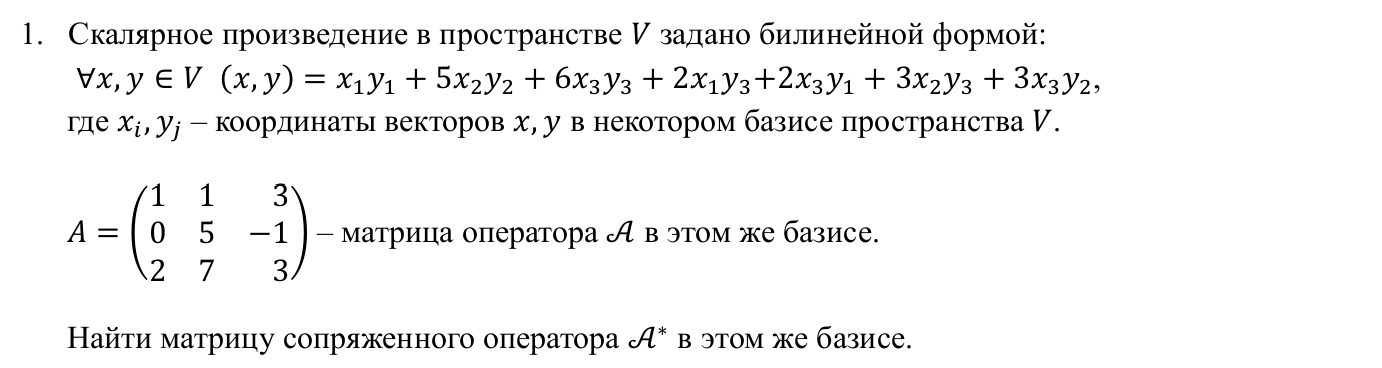
\includegraphics{assets/practice-6-task-1.png}
\end{center}
\textbf{Решение:}

Напишем матрицу Грама:$\begin{pmatrix}
    1 & 0 & 2 \\
    0 & 5 & 3 \\
    2 & 3 & 6
\end{pmatrix}$. $A^\circledast = \overline{\Gamma^{-1}}A^* \overline{\Gamma} = \Gamma^{-1}A^T \Gamma$. Считаем и побеждаем.

\subsubsection{Задание 2.}

\begin{center}
   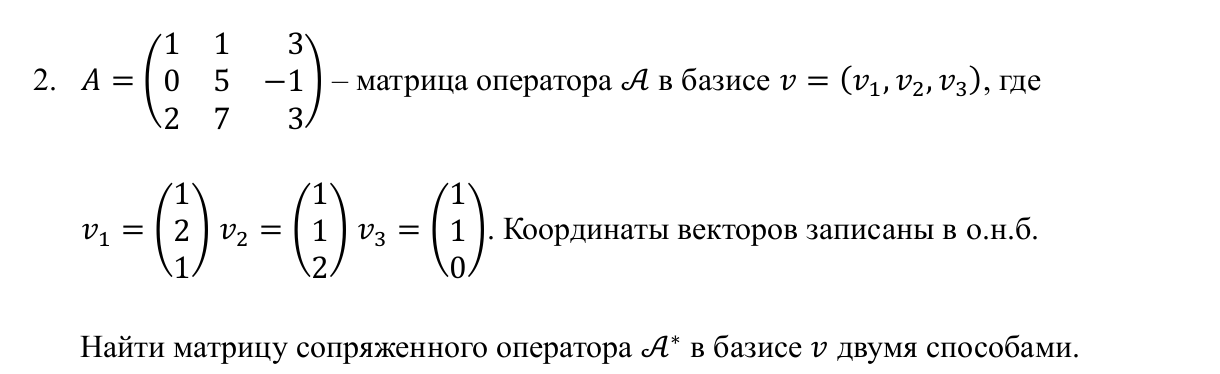
\includegraphics{assets/practice-6-task-2.png}
\end{center}

\textbf{Решение:}

Можно решить двумя способами: $A^\circledast_v = T^{-1}A_e^\circledast T$, либо $A^\circledast_v = \Gamma_v^{-1}A_v^T \Gamma_v$

\subsubsection{Задание 3.}

\begin{center}
   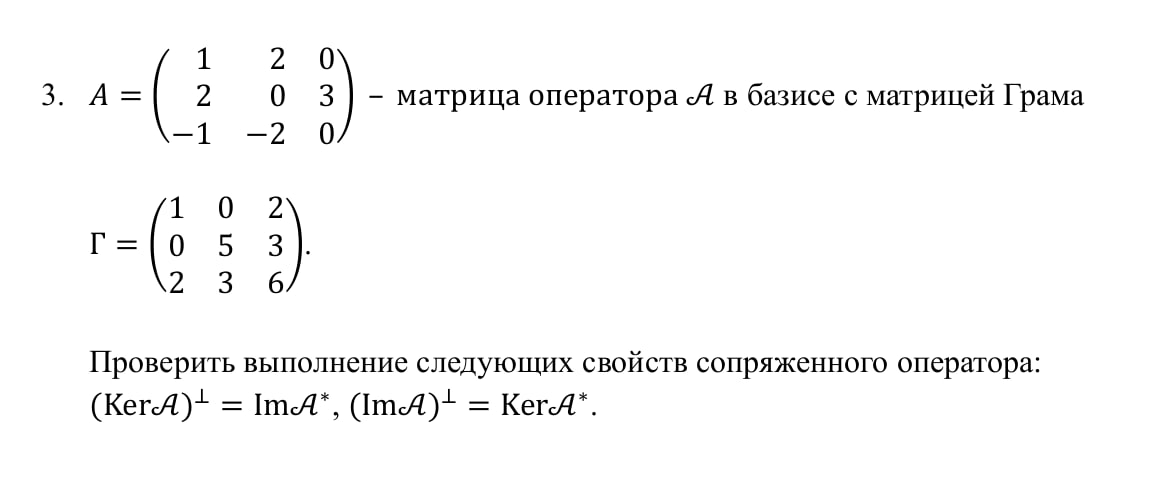
\includegraphics[width = 15 cm]{assets/practice-6-task-3.png}
\end{center}

не думаю, что тут стоит что-либо писать, так как это просто комбинация прошлых задач.
